\documentclass[11pt]{article}
\usepackage[margin=0.75in]{geometry}
\usepackage{graphicx}
\usepackage{amsmath}
\usepackage{hyperref}
\usepackage{enumitem}
\usepackage{tikz}
\usepackage{xcolor}
\usetikzlibrary{shapes,arrows,positioning,fit,backgrounds}

\title{\textbf{Solstice: Automated Fact-Checking for Medical Documentation}}
\author{A Multi-Agent System for Evidence Extraction and Verification}
\date{}

\begin{document}
\maketitle

\section{Overview}

Solstice is an automated system for fact-checking medical claims against scientific literature. It processes PDFs through a pipeline that combines layout detection, content extraction, and multi-agent verification to produce comprehensive evidence reports.

\section{System Architecture}

The Solstice pipeline consists of five main stages:

\begin{enumerate}
\item \textbf{PDF Input}: Medical documents including clinical trials, package inserts, and marketing materials
\item \textbf{Layout Detection}: Computer vision models identify document structure (text blocks, tables, figures)
\item \textbf{Content Extraction}: Structured extraction of text and visual elements
\item \textbf{Multi-Agent Analysis}: LLM-based agents extract and verify evidence
\item \textbf{Report Generation}: Consolidated evidence reports with confidence assessments
\end{enumerate}

\section{How It Works}

\subsection{Step 1: Understanding Document Structure}

Medical documents are complex—they mix narrative text with data tables, clinical figures, and regulatory disclaimers. Solstice first "sees" the document using computer vision to identify each element:

\begin{figure}[htbp]
\centering
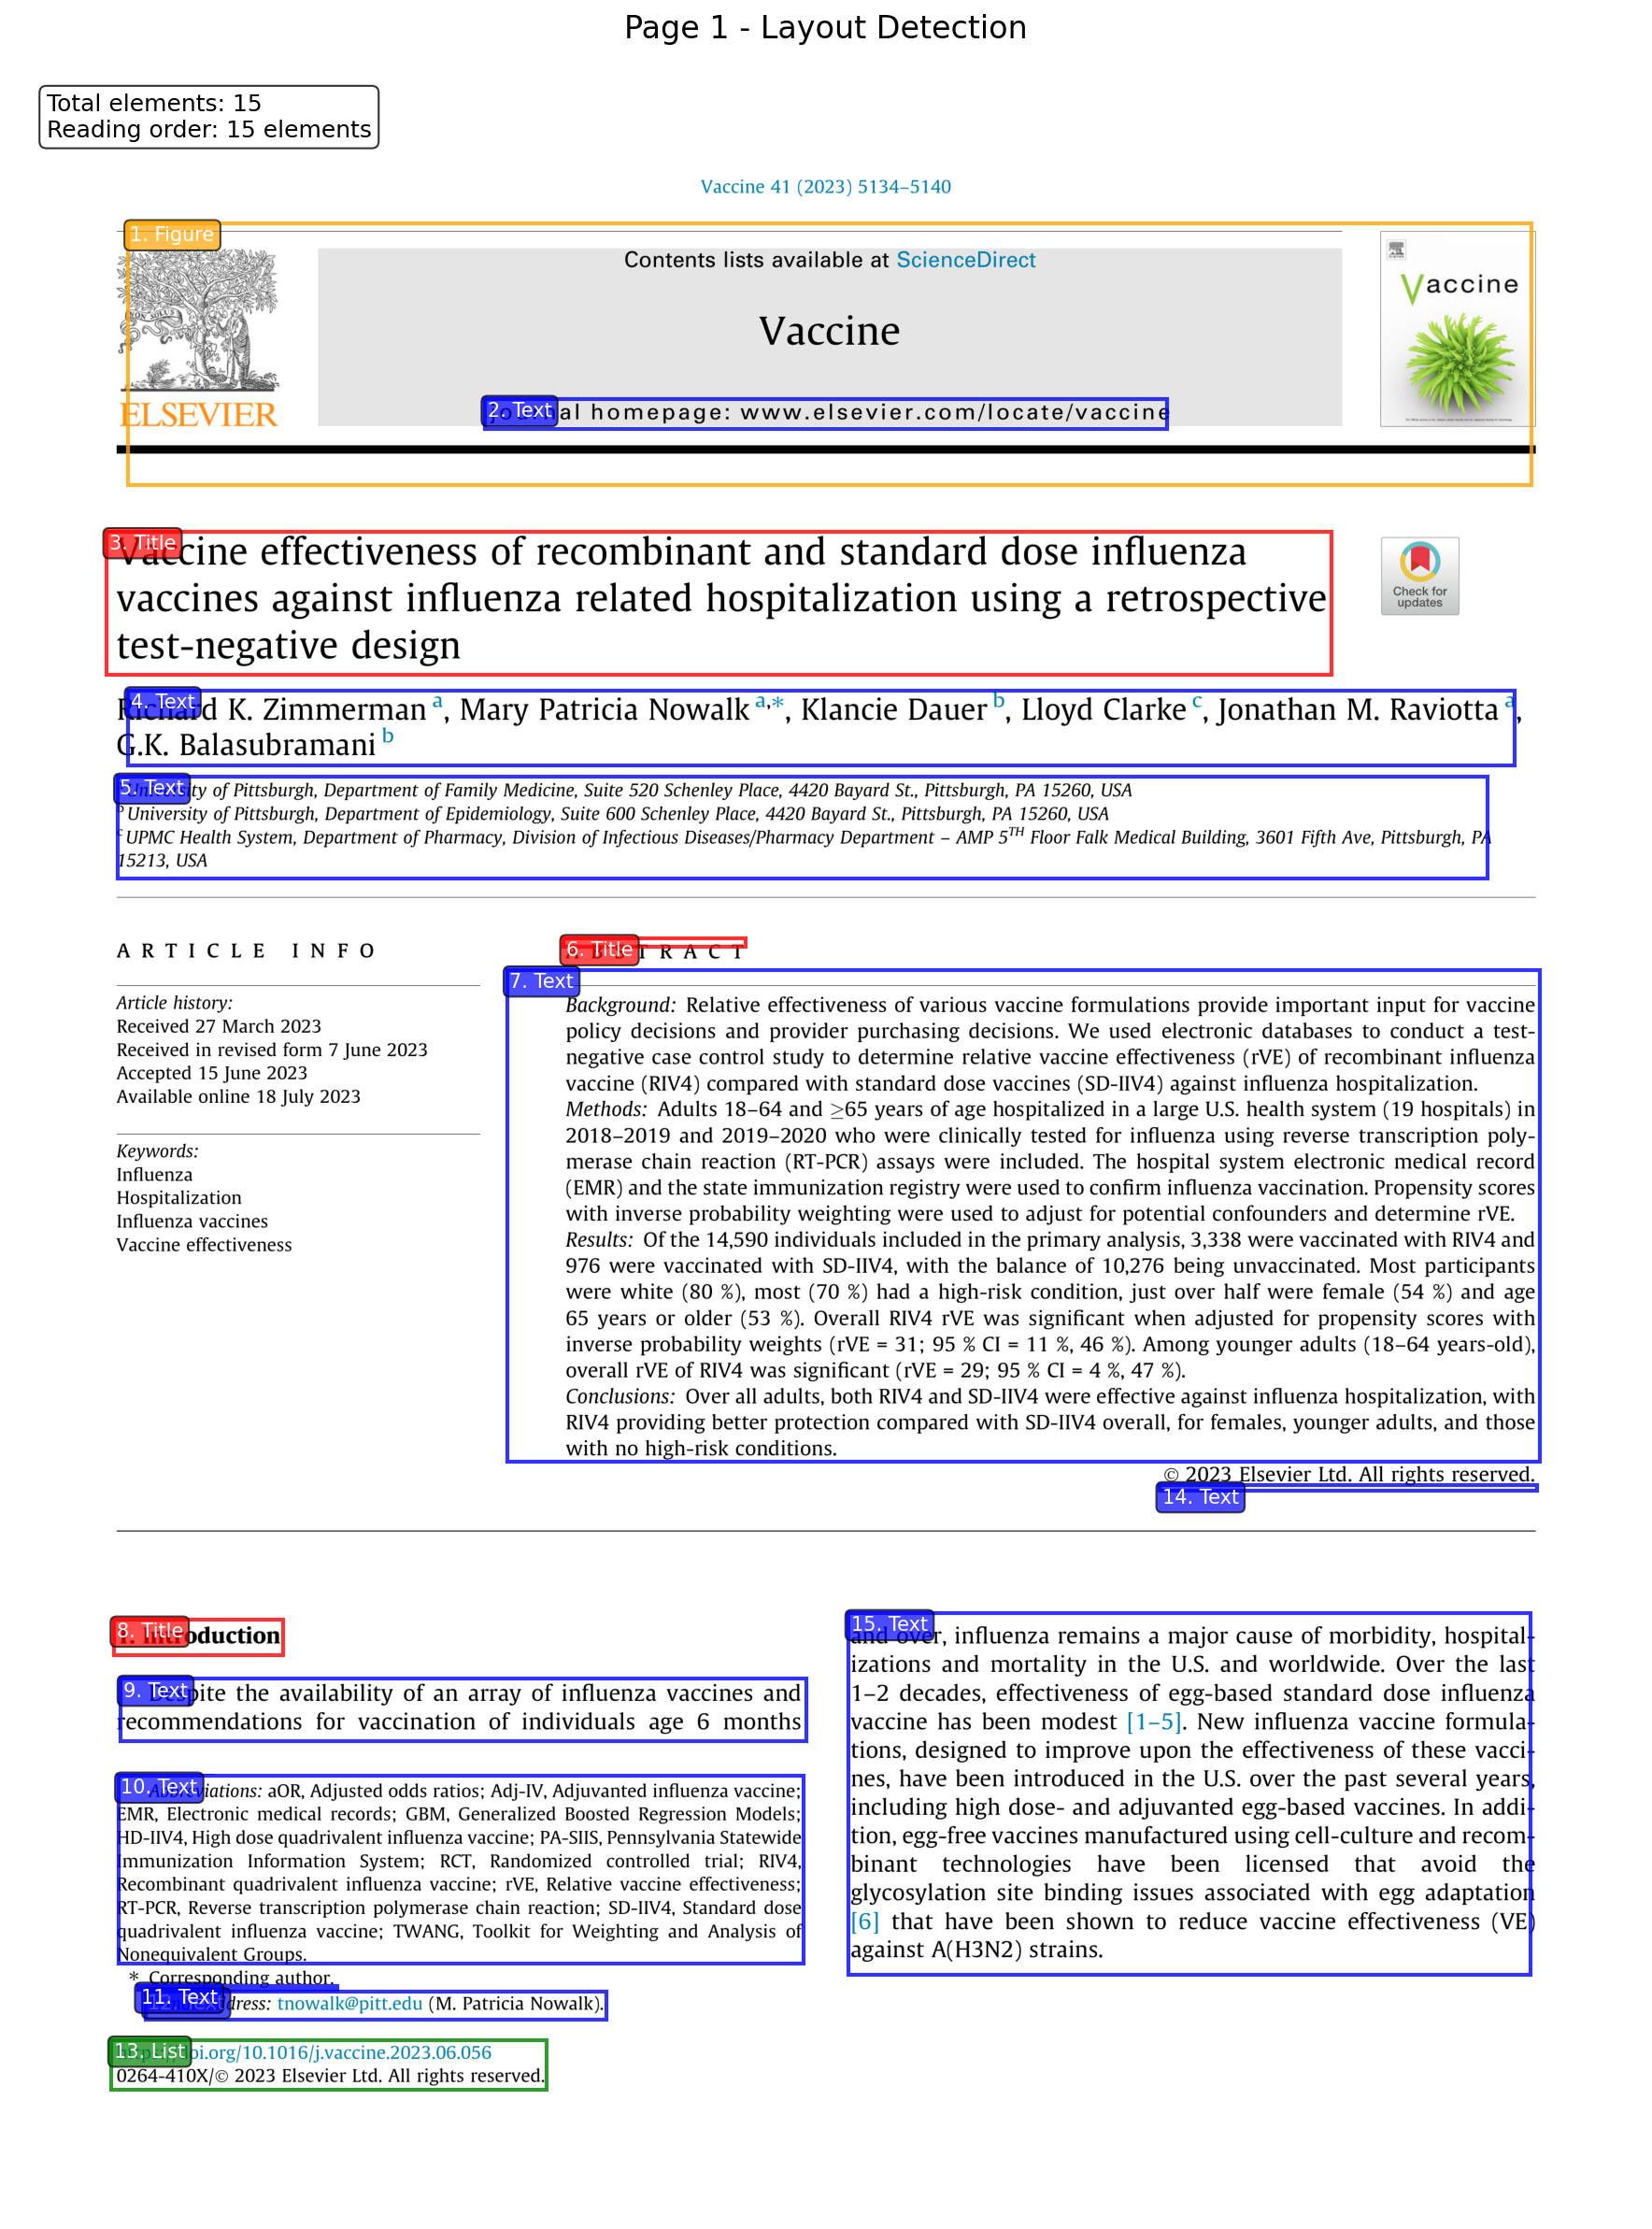
\includegraphics[width=0.85\textwidth]{scientific_layout_example.png}
\caption{Layout detection on a clinical trial paper identifies distinct regions: title, abstract, body text, tables, and figures. Each element is extracted separately for targeted analysis.}
\end{figure}

This visual understanding is crucial because:
\begin{itemize}
\item Key efficacy data often appears in tables
\item Safety information may be in figure captions
\item Important disclaimers hide in footnotes
\item Marketing materials use visual hierarchy to emphasize claims
\end{itemize}

\subsection{Step 2: Multi-Agent Verification}

Once documents are structured, four specialized agents collaborate to verify claims:

The agent pipeline processes claims through multiple stages:

\begin{enumerate}
\item \textbf{Evidence Extractor}: Searches documents for passages related to the claim
\item \textbf{Evidence Verifier}: Confirms quotes are accurate and truly support the claim  
\item \textbf{Completeness Checker}: Identifies missing evidence and triggers additional searches
\item \textbf{Visual Analyzer}: Examines tables and figures for data supporting or contradicting claims
\end{enumerate}

Agents communicate through structured JSON outputs, with feedback loops allowing the Completeness Checker to request additional extraction when gaps are identified.

\section{Real-World Applications}

\subsection{Clinical Trial Verification}
When pharmaceutical companies publish trial results, Solstice can verify that marketing claims accurately reflect the scientific data. The system catches discrepancies like selective reporting or overgeneralization of results.

\subsection{Regulatory Compliance}
Medical device manufacturers must ensure their promotional materials align with FDA-approved indications. Solstice automatically cross-references marketing claims against regulatory documents.

\subsection{Marketing Material Review}

Marketing materials require special attention due to their persuasive nature:

\begin{figure}[htbp]
\centering
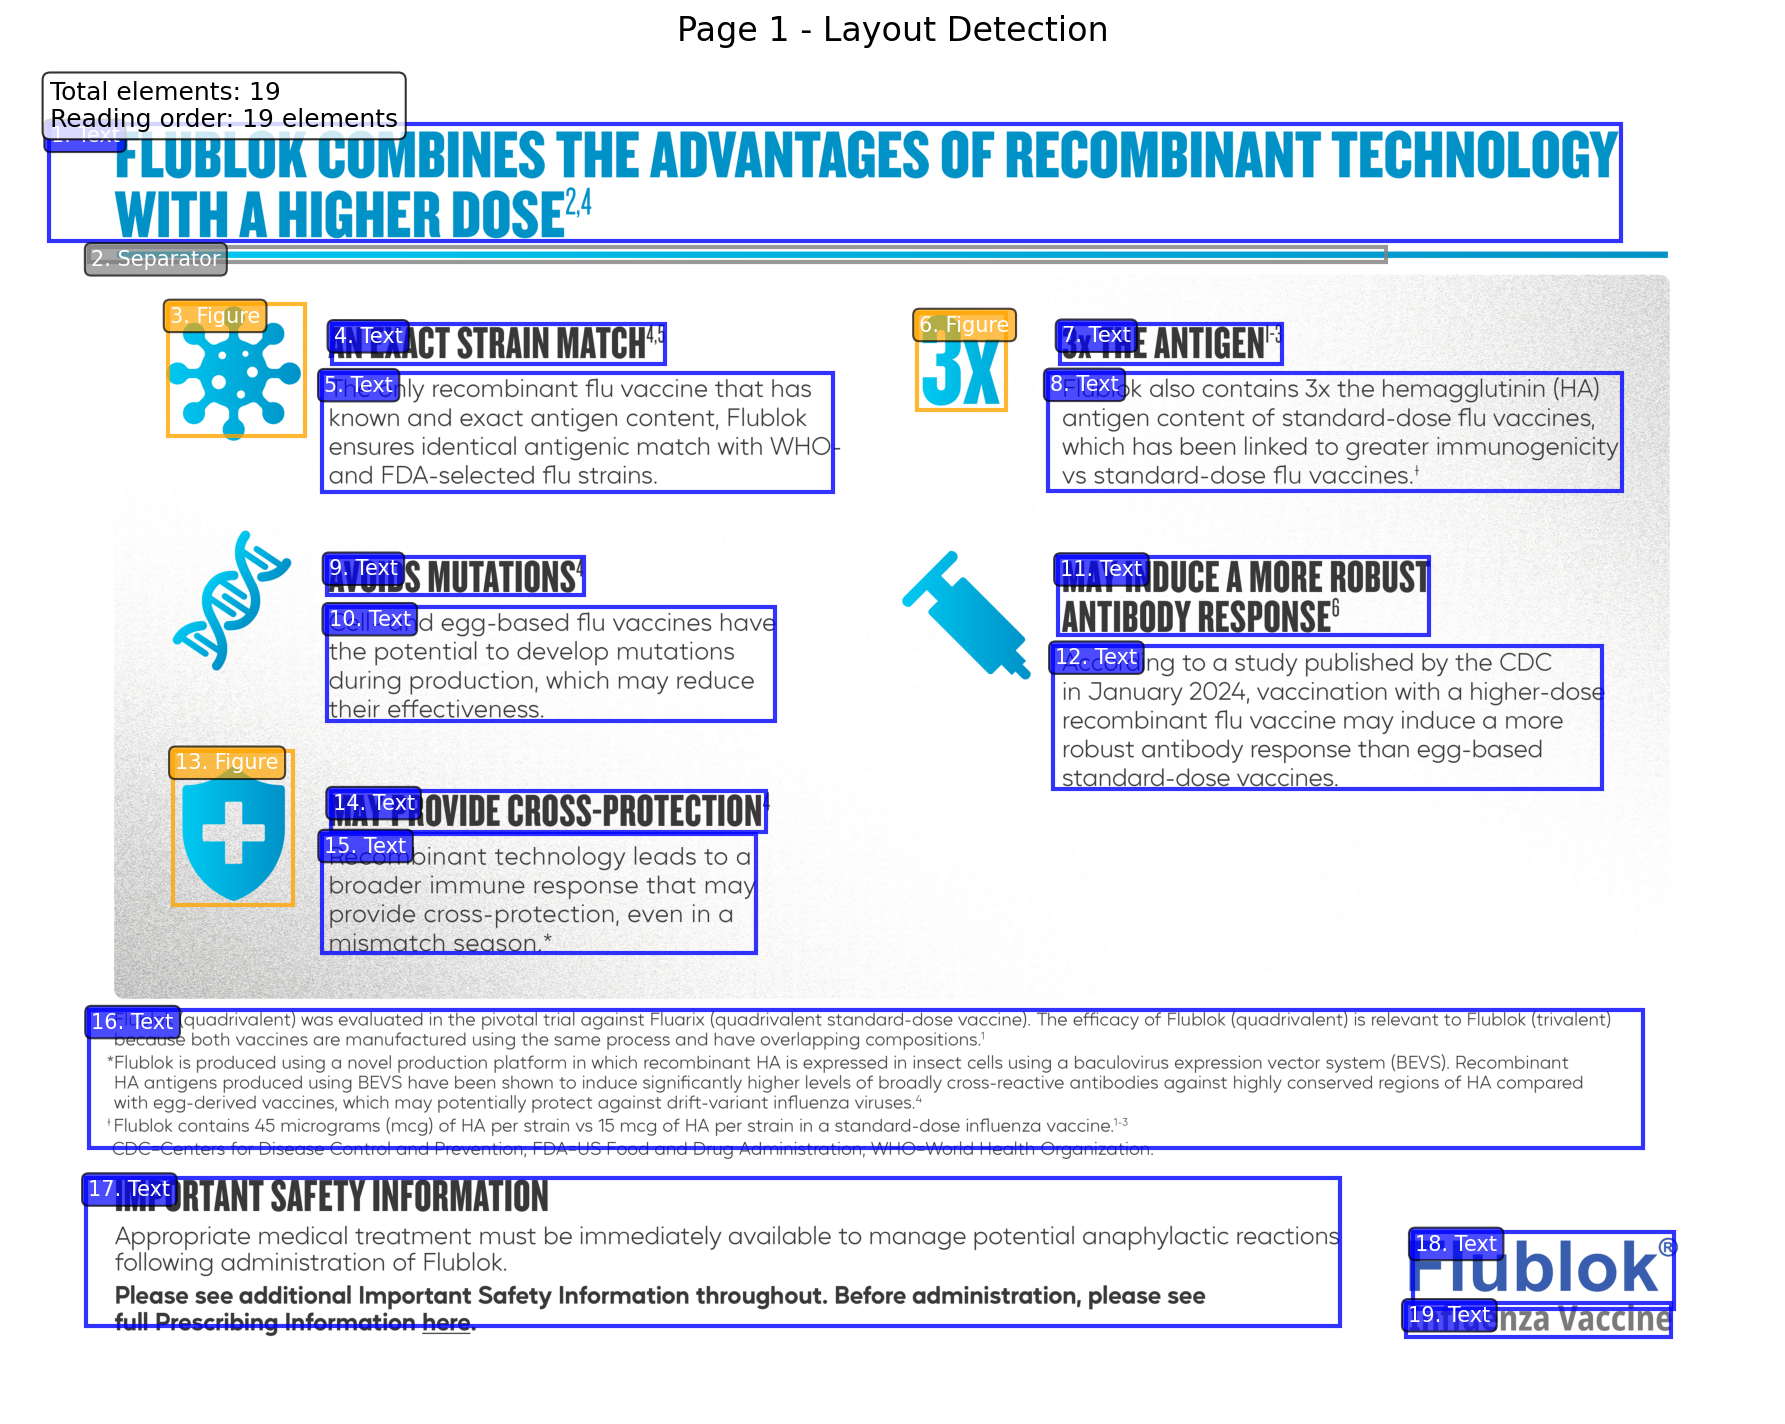
\includegraphics[width=0.85\textwidth]{marketing_layout_example.png}
\caption{Marketing materials use visual design to emphasize benefits. Solstice identifies promotional claims and verifies them against clinical evidence.}
\end{figure}

\section{Key Innovations}

\subsection{Multimodal Understanding}
Unlike text-only systems, Solstice analyzes tables, graphs, and figures—critical for medical evidence where key data often appears visually.

\subsection{Intelligent Orchestration}
Agents work together with feedback loops, ensuring thorough verification. If gaps are found, the system automatically searches for additional evidence.

\subsection{Traceable Verification}
Every claim links back to its source evidence, maintaining transparency and allowing human review of the automated findings.

\subsection{Scalable Architecture}
The system processes multiple claims in parallel while managing computational resources efficiently.

\section{Impact and Benefits}

\begin{itemize}
\item \textbf{Speed}: Reduces verification time from days to minutes
\item \textbf{Accuracy}: Systematic analysis eliminates human oversight errors
\item \textbf{Completeness}: Examines entire documents, not just keyword matches
\item \textbf{Transparency}: Provides traceable evidence for every verification
\item \textbf{Scalability}: Handles large document sets that would overwhelm human reviewers
\end{itemize}

\section{Future Directions}

Solstice continues to evolve with planned enhancements:
\begin{itemize}
\item Cross-document reasoning to synthesize evidence from multiple sources
\item Temporal analysis to track how claims change over time
\item Contradiction detection between related documents
\item Integration with regulatory databases for real-time compliance checking
\end{itemize}

\section{Conclusion}

Solstice represents a paradigm shift in medical document verification. By combining visual document understanding with intelligent agent orchestration, it transforms a manual, error-prone process into an automated, reliable system. This enables faster drug development, more accurate marketing, and ultimately, better-informed healthcare decisions.

\end{document}